\chapter{流形的基本概念}
\label{chap:manifold-basics}
\label{chap:differential-geometry-and-symmetry}

在地球表面上记录位置，常用经度和纬度。这套坐标在大部分地方很好用，到了两极却出了问题：北极点的经度可以取任意值，所以经纬度不是这一点的唯一记录；沿纬线绕北极走一圈，经度从$\pi$跳回$-\pi$，走的路连续，记录却断了。图~\ref{fig:mfd-latlong}把这两处毛病画在一起。

\begin{BookInlineFigure}
  \centering
  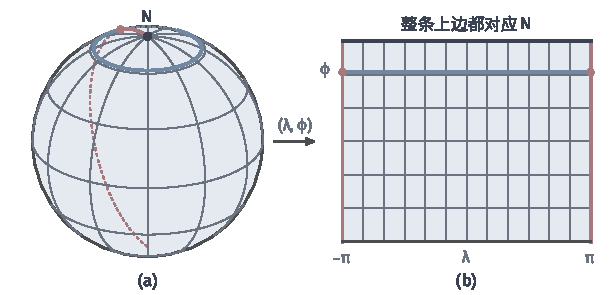
\includegraphics[width=104mm]{figures/04-spaces-measures-and-geometry/04-manifolds/matplotlib/mfd-sphere-latlong/figure.pdf}
  \caption{经纬度为什么覆盖不了整个球面。(a)球面上的经纬网，蓝色是高纬度的一条纬线，红色是取作接缝的经线$\lambda=\pm\pi$，背面部分画成虚线。(b)同一套网格在坐标矩形$(\lambda,\phi)$中的样子：北极一点被拉成整条上边，接缝被切成左右两条红边。球面上闭合的蓝色纬线在矩形中成为一条线段，两个红点是接缝上的同一点。}
  \label{fig:mfd-latlong}
\end{BookInlineFigure}

地图册解决这类问题的办法是用很多张局部地图拼起来：每张图只负责一块区域，在这块区域内干净地记录位置；相邻的图在重叠处约定怎样换算。圆周也是这样，一个角度足以定位一小段圆弧上的点，却无法不重复、不跳跃地记录整个圆。

这类对象的共同点是“局部像欧氏空间，整体未必是”。本章把这一认识写成\term{流形}（manifold）的定义，全程用圆、球面和环面三个具体对象走一遍：先用坐标图和换算规则定义流形，看局部欧氏结构带来哪些拓扑性质；再在流形上区分点、曲线、切向量和余切向量；然后建立随点变化的函数与场，最后用单位分解把局部构造拼成整体。

有一条线索贯穿全章：坐标是记录，不是对象。同一点、同一个速度、同一个读数在不同的图里有不同的数，这些数之间的换算规则由图之间的转移映射决定。凡是想在流形上定义一个概念，都要回答两个问题：它在一张图里怎么写，换一张图时结论是否不变。

本章只讨论同一个流形内部的对象。一个流形到另一个流形的映射怎样作用于点和切向量，是第~\ref{chap:manifold-maps}章的问题；两个流形何时光滑等价、何时构成子流形，见第~\ref{chap:manifold-relations}章。长度和角度需要额外选取度量，见第~\ref{chap:riemannian-geometry}章；微分形式与积分见第~\ref{chap:manifold-calculus}章。所用的拓扑概念沿用第~\ref{chap:topological-spaces}章。

\section{流形的定义}
\label{sec:mfd-definition}

曲线和曲面在微积分里常由参数化给出：圆是$\theta\mapsto(\cos\theta,\sin\theta)$的像，球面可以用经纬度参数化。参数化把一块欧氏区域送到对象上；反过来读，就是用几个实数记录对象上的一个点。图~\ref{fig:mfd-latlong}说明一张参数化通常只能照顾一部分，所以我们需要多张局部记录，并规定它们在重叠处怎样换算。

\subsection{坐标图与光滑相容性}
\label{sec:mfd-charts-compatibility}

先看圆周
\[
S^1=\{\bm y\in\mathbb R^2:\lVert\bm y\rVert_2=1\}.
\]
角度$\theta$可以记录圆上的点，但取值范围必须选一个长度为$2\pi$的开区间，否则同一点会有两个角度。取$(-\pi,\pi)$时，点$(-1,0)$没有角度；取$(0,2\pi)$时，点$(1,0)$没有角度。

为什么不用半开区间$[-\pi,\pi)$把漏掉的点补上？因为那样记录就不连续了：从下方逼近$(-1,0)$的点，角度趋于$-\pi$；从上方逼近的点，角度趋于$\pi$。圆上挨得很近的两点，记录却相距接近$2\pi$。单个角度无论怎样选，不是漏点就是断开，必须用至少两张局部记录才能覆盖整个圆。

\paragraph{坐标图与图册}
把“局部记录”说准确。它应当做两件事：把一块区域一一对应到欧氏空间的开集，并且不破坏邻近关系。这正是同胚的要求，即连续的双射且逆映射也连续。于是坐标接近当且仅当点接近，上面半开区间的毛病被排除在外。

\begin{definition}[坐标图与图册]
\label{def:mfd-chart}
设$M$是拓扑空间，$n\geq0$为整数。若$U\subseteq M$是开集，$\varphi:U\to\widehat U$是从$U$到某个开集$\widehat U\subseteq\mathbb R^n$的同胚，则称$(U,\varphi)$为$M$的一张$n$维\term{坐标图}（chart），$U$为它的定义域。对$p\in U$，称
\begin{equation}
\varphi(p)=(x_1(p),\ldots,x_n(p))
\label{eq:mfd-chart-coordinates}
\end{equation}
为$p$在这张图中的坐标，实值函数$x_i:U\to\mathbb R$称为坐标函数。定义域覆盖$M$的一族坐标图称为\term{图册}（atlas）。
\end{definition}

这些名词就是地图册的术语。表~\ref{tab:mfd-atlas-analogy}列出对应关系。类比在一处需要小心：真实的地图印在纸上有边缘和比例尺，坐标图只保证拓扑上的忠实，既不保持距离也不保持角度。距离要等到第~\ref{chap:riemannian-geometry}章选定度量之后才有意义。

\begin{BookInlineTable}
  \centering
  \begin{tabular}{ll}
    \toprule
    地图册 & 流形\\
    \midrule
    地球表面 & 空间$M$\\
    地面上的地点 & 点$p\in M$\\
    一张地图覆盖的区域 & 开集$U\subseteq M$\\
    把地点标到纸上的规则 & 同胚$\varphi:U\to\widehat U$\\
    地点在图上的位置 & 坐标$\varphi(p)$\\
    相邻两图的换算表 & 转移映射$\psi\circ\varphi^{-1}$\\
    \bottomrule
  \end{tabular}
  \caption{地图册与流形术语的对应。}
  \label{tab:mfd-atlas-analogy}
\end{BookInlineTable}

圆周的两张角度图组成一个图册：
\begin{equation}
\theta_1:S^1\setminus\{(-1,0)\}\to(-\pi,\pi),\qquad
\theta_2:S^1\setminus\{(1,0)\}\to(0,2\pi).
\label{eq:mfd-circle-charts}
\end{equation}
两者的逆都是$\theta\mapsto(\cos\theta,\sin\theta)$在相应区间上的限制。图的方向是“点到坐标”，参数化的方向是“坐标到点”，二者互为逆映射。图~\ref{fig:mfd-circle-charts}的(a)(b)画出了这两张图各漏掉哪一点。

\begin{BookInlineFigure}
  \centering
  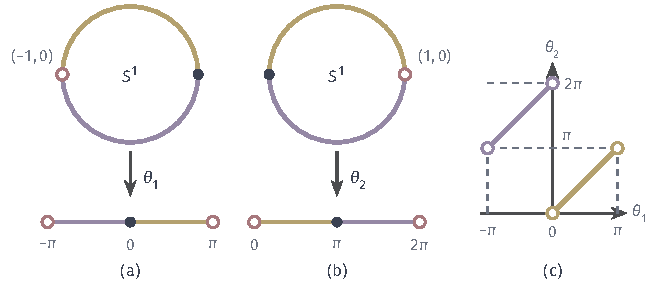
\includegraphics[width=111.605mm]{figures/04-spaces-measures-and-geometry/04-manifolds/tikz/mfd-circle-charts/figure.pdf}
  \caption{圆周的两张角度图及其转移映射。(a)(b)$\theta_1$漏掉$(-1,0)$，$\theta_2$漏掉$(1,0)$，漏掉的点用空心红圈表示。黄色弧是上半圆，紫色弧是下半圆，下方的开区间用相同颜色标出它们的坐标。(c)在重叠部分，$\theta_2$作为$\theta_1$的函数：上半圆上$\theta_2=\theta_1$（黄），下半圆上$\theta_2=\theta_1+2\pi$（紫），空心点表示这些坐标不属于重叠部分。}
  \label{fig:mfd-circle-charts}
\end{BookInlineFigure}

\paragraph{拓扑流形}
有了坐标图，就可以说一个空间“局部像$\mathbb R^n$”：每点都落在某张$n$维坐标图的定义域中。只要求这一条还不够，定义中要另加两个拓扑条件，用来排除两类病态空间。

\begin{definition}[拓扑流形]
\label{def:mfd-topological-manifold}
拓扑空间$M$称为$n$维\term{拓扑流形}（topological manifold），若它满足：
\begin{enumerate}
\item $M$是Hausdorff空间：任意两个不同点有互不相交的邻域；
\item $M$是第二可数的：拓扑有一个可数的基；
\item $M$局部欧氏：每个$p\in M$都属于某张$n$维坐标图的定义域。
\end{enumerate}
\end{definition}

Hausdorff条件保证点列的极限唯一。去掉它，就可能出现“双原点直线”：取两条实轴，把除原点以外的同名点粘在一起。所得空间每点附近都像一段实轴，局部欧氏条件成立；但两个原点没有不相交的邻域，点列$1/k$同时收敛到这两个原点。

第二可数条件排除“太大”的空间，例如不可数多条互不相交的实轴之并。这个条件有实际用途：它保证流形只有可数个连通分支，并能用一列紧集逐步穷竭，第~\ref{sec:mfd-partition-unity}节构造单位分解时就要用到。两个条件的一般讨论见第~\ref{chap:topological-spaces}章。

\paragraph{坐标变换与光滑相容}
拓扑流形只告诉我们哪些点彼此接近，还不能说一个函数“可微”。自然的想法是把函数写到坐标里再求导，但同一点可能落在两张图中，两张图的结论必须一致。这就要考察两套坐标之间的换算。

设$(U,\varphi)$与$(V,\psi)$是两张坐标图，$U\cap V\neq\varnothing$。先用$\varphi^{-1}$从第一张图回到流形上的点，再用$\psi$记到第二张图上，得到映射
\begin{equation}
\psi\circ\varphi^{-1}:\varphi(U\cap V)\to\psi(U\cap V).
\label{eq:mfd-transition}
\end{equation}
它把同一点在第一张图中的坐标换成第二张图中的坐标，称为\term{坐标变换}（transition map），也叫转移映射。

图~\ref{fig:mfd-chart-transition}画出了这个过程。要留意的是：$\varphi$和$\psi$的定义域在流形上，流形上一般没有微积分；而转移映射的定义域和值域都在欧氏空间里，可以用多元微积分判断它是否可微。这就是定义光滑结构的切入点。

\begin{BookInlineFigure}
  \centering
  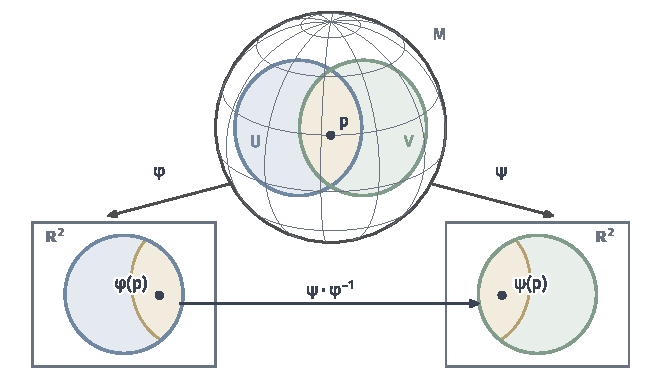
\includegraphics[width=112mm]{figures/04-spaces-measures-and-geometry/04-manifolds/matplotlib/mfd-chart-transition/figure.pdf}
  \caption{两张坐标图与转移映射。上方是球面上的两个球冠$U$（蓝）和$V$（绿），重叠部分为黄色。下方分别是向球冠中心切平面作正交投影得到的两张图。黄色区域是同一块重叠部分在两张图中的像，形状不同；转移映射$\psi\circ\varphi^{-1}$在两个黄色区域之间换算同一点$p$的坐标。}
  \label{fig:mfd-chart-transition}
\end{BookInlineFigure}

\begin{definition}[光滑相容与光滑结构]
\label{def:mfd-smooth-structure}
两张$n$维坐标图$(U,\varphi)$与$(V,\psi)$称为\term{光滑相容}（smoothly compatible）的，若$U\cap V=\varnothing$，或者坐标变换$\psi\circ\varphi^{-1}$与其逆$\varphi\circ\psi^{-1}$都是无穷次连续可微的。任意两张图都光滑相容的图册称为光滑图册。若一个光滑图册包含了所有与它的每张图都光滑相容的坐标图，就称它为极大光滑图册，也称$M$上的一个\term{光滑结构}（smooth structure）。带有光滑结构的拓扑流形称为\term{光滑流形}（smooth manifold）。
\end{definition}

本书说“光滑”都指无穷次连续可微。定义要求转移映射和它的逆都光滑，因为一个方向光滑不能保证另一方向也光滑，稍后的$x\mapsto x^3$就是例子。

极大图册听起来很大，实际使用时只需给出一个光滑图册：所有与它光滑相容的坐标图放在一起，就是包含它的唯一极大图册。需要检查的是这些新加入的图彼此也光滑相容。设$(V_1,\psi_1)$与$(V_2,\psi_2)$都与原图册相容，$q\in V_1\cap V_2$，取原图册中包含$q$的图$(U,\varphi)$。在$\psi_1(q)$附近可以经由$\varphi$中转：
\[
\psi_2\circ\psi_1^{-1}=(\psi_2\circ\varphi^{-1})\circ(\varphi\circ\psi_1^{-1}).
\]
右端两个因子都光滑，所以左端在$\psi_1(q)$附近光滑。光滑性是局部性质，逐点成立就在整个重叠区域成立。今后说“$M$的坐标图”，都指光滑结构中的坐标图。

\paragraph{例子：圆周}
现在把定义在圆周上走一遍。重叠区域是去掉$(\pm1,0)$后的两段开半圆。在上半圆，两个角度取值相同；在下半圆，$\theta_1$取$(-\pi,0)$中的值，$\theta_2$取$(\pi,2\pi)$中的值，二者相差$2\pi$。所以
\begin{equation}
\theta_2\circ\theta_1^{-1}(s)=
\begin{cases}
s, & s\in(0,\pi),\\
s+2\pi, & s\in(-\pi,0).
\end{cases}
\label{eq:mfd-circle-transition}
\end{equation}
图~\ref{fig:mfd-circle-charts}(c)是这个函数的图像，两段都是斜率为$1$的线段。

式~\eqref{eq:mfd-circle-transition}的定义域由两个不相交的开区间组成，在每段上都是平移，所以光滑，它的逆也是平移。于是这两张图构成光滑图册。坐标在下半圆跳过$2\pi$，只是记录方式的变化，圆本身并没有在那里断开。图中两段线段之间的空隙对应$\theta_1=0$，那里是$(1,0)$，它不在$\theta_2$的定义域内，所以不属于重叠部分。

\paragraph{例子：球面}
单位球面$S^2=\{\bm y\in\mathbb R^3:\lVert\bm y\rVert_2=1\}$上最方便的两张图来自\term{球极投影}（stereographic projection）。记北极$N=(0,0,1)$、南极$S=(0,0,-1)$。从北极向球面上的点$\bm y$作射线，射线与赤道平面的交点就是$\bm y$的坐标，如图~\ref{fig:mfd-stereographic}(a)所示。

下面把这个几何作图写成公式。过$N$和$\bm y$的直线上的点是$N+t(\bm y-N)$，它的第三个分量是$1+t(y_3-1)$。令第三个分量为零，得到
\[
t=\frac{1}{1-y_3}.
\]
代回前两个分量，得到北极图
\begin{equation}
\sigma_N(\bm y)=\frac{(y_1,y_2)}{1-y_3},\qquad \bm y\in S^2\setminus\{N\}.
\label{eq:mfd-stereographic-north}
\end{equation}

\begin{BookInlineFigure}
  \centering
  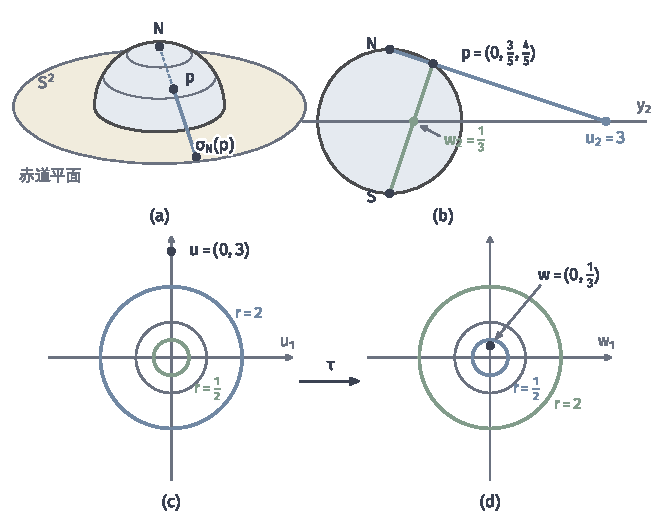
\includegraphics[width=112mm]{figures/04-spaces-measures-and-geometry/04-manifolds/matplotlib/mfd-stereographic/figure.pdf}
  \caption{球极投影及其转移映射。(a)从北极$N$过球面点$p$的射线交赤道平面（黄）于$\sigma_N(p)$，球内部分用虚线。(b)过$N$和$p=(0,\tfrac35,\tfrac45)$的竖直截面，蓝线给出北极图坐标$u_2=3$，绿线从南极给出南极图坐标$w_2=\tfrac13$。(c)(d)转移映射$\tau$把$\bm u$平面的圆周送到$\bm w$平面：半径$2$的蓝圆变成半径$\tfrac12$，半径$\tfrac12$的绿圆变成半径$2$，单位圆不变，$(0,3)$变成$(0,\tfrac13)$。}
  \label{fig:mfd-stereographic}
\end{BookInlineFigure}

反过来，给定$\bm u\in\mathbb R^2$，求球面上的对应点。记$\rho=\lVert\bm u\rVert_2^2$，点$\sigma_N^{-1}(\bm u)$在从$N$到$(\bm u,0)$的线段上，形如$(s\bm u,1-s)$。它在球面上，于是
\[
s^2\rho+(1-s)^2=1 .
\]
展开后约去$s\neq0$，得到$s(\rho+1)=2$。把$s=2/(\rho+1)$代回，就得到
\begin{equation}
\sigma_N^{-1}(\bm u)=\frac{\bigl(2u_1,\;2u_2,\;\rho-1\bigr)}{\rho+1},\qquad \rho=\lVert\bm u\rVert_2^2 .
\label{eq:mfd-stereographic-inverse}
\end{equation}
这是有理函数，$\sigma_N$与它的逆都连续，所以$\sigma_N$是$S^2\setminus\{N\}$到整个$\mathbb R^2$的同胚。同样地，从南极投影得到南极图
\begin{equation}
\sigma_S(\bm y)=\frac{(y_1,y_2)}{1+y_3},\qquad \bm y\in S^2\setminus\{S\}.
\label{eq:mfd-stereographic-south}
\end{equation}

两张图的重叠区域是去掉两极的球面，对应北极图中的$\mathbb R^2\setminus\{\bm0\}$。把式~\eqref{eq:mfd-stereographic-inverse}代入$\sigma_S$，先算分母：
\[
1+y_3=1+\frac{\rho-1}{\rho+1}=\frac{2\rho}{\rho+1}.
\]
前两个分量是$2\bm u/(\rho+1)$，相除后$\rho+1$消去，得到转移映射
\begin{equation}
\tau(\bm u)=\sigma_S\circ\sigma_N^{-1}(\bm u)=\frac{\bm u}{\lVert\bm u\rVert_2^2},\qquad \bm u\neq\bm 0.
\label{eq:mfd-stereographic-transition}
\end{equation}
这个映射叫反演：方向不变，半径变成倒数，图~\ref{fig:mfd-stereographic}(c)(d)就是它的样子。

$\tau$在$\mathbb R^2\setminus\{\bm0\}$上光滑，因为它是分母不为零的有理函数。再算$\tau\circ\tau$。由范数的计算，
\[
\lVert\tau(\bm u)\rVert_2^2=\frac{1}{\lVert\bm u\rVert_2^2},
\]
所以$\tau(\tau(\bm u))=\bm u$，$\tau$的逆就是它自己，同样光滑。于是$\{\sigma_N,\sigma_S\}$是$S^2$的光滑图册。球面作为$\mathbb R^3$的子空间，Hausdorff性与第二可数性都从$\mathbb R^3$继承，因此是二维光滑流形。

\paragraph{例子：欧氏开集与乘积}
最简单的光滑流形是$\mathbb R^n$本身，用恒等映射作唯一的图。它的任意开子集$W$也是光滑流形，图为恒等映射在$W$上的限制。更一般地，光滑流形的开子集用原有坐标图限制到其中，就成为同维光滑流形。

两个流形可以相乘。设$M$与$N$分别是$m$维与$n$维光滑流形，$(U,\varphi)$与$(V,\psi)$分别是二者的坐标图，令
\begin{equation}
(\varphi\times\psi)(p,q)=(\varphi(p),\psi(q))\in\mathbb R^{m+n}.
\label{eq:mfd-product-chart}
\end{equation}
这些乘积图覆盖$M\times N$。两张乘积图之间的坐标变换是两个坐标变换并排作用，各自光滑，所以并排后也光滑。乘积拓扑仍是Hausdorff且第二可数的，于是$M\times N$是$m+n$维光滑流形，称为\term{乘积流形}（product manifold）。

\term{环面}（torus）$T^2=S^1\times S^1$是最常用的乘积例子。一点由两个角度$(\theta,\phi)$记录，图~\ref{fig:mfd-torus-product}左边的正方形就是角度的取值范围，右边是同一个流形放进$\mathbb R^3$的样子，公式为
\[
\bigl((2+r\cos\phi)\cos\theta,\ (2+r\cos\phi)\sin\theta,\ r\sin\phi\bigr),\quad 0<r<2 .
\]
这只是外观，环面作为乘积流形并不需要$\mathbb R^3$。正方形的上下边是同一个圆，左右边也是同一个圆，把两组对边粘起来就得到环面。

\begin{BookInlineFigure}
  \centering
  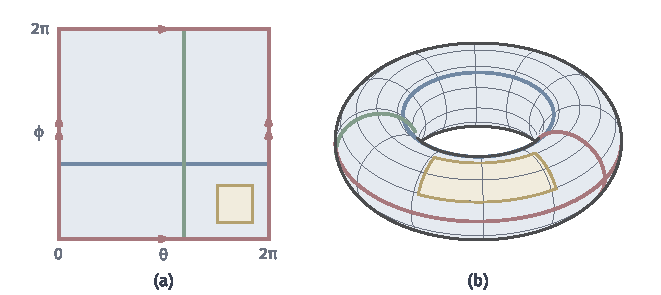
\includegraphics[width=112mm]{figures/04-spaces-measures-and-geometry/04-manifolds/matplotlib/mfd-torus-product/figure.pdf}
  \caption{环面$S^1\times S^1$的角度坐标。(a)角度正方形，带箭头的红色对边两两等同；黄色矩形是一小块坐标区域，蓝线$\phi=$常数，绿线$\theta=$常数。(b)嵌入$\mathbb R^3$的环面（$r=0.82$）上同一块区域和同样两条圈，红色两条圈是$\phi=0$和$\theta=0$的接缝。灰线为角度网格。}
  \label{fig:mfd-torus-product}
\end{BookInlineFigure}

圆周的两张图做乘积，就得到环面的四张图：$\theta_a\times\theta_b$，$a,b\in\{1,2\}$。以圆周上$\theta_1=1$和$\theta_1=-2$对应的两点组成的乘积点为例，它在四张图中的坐标分别是
\[
(1,-2),\quad (1,-2+2\pi),\quad (1,-2),\quad (1,-2+2\pi),
\]
依次对应$(a,b)=(1,1),(1,2),(2,1),(2,2)$，其中第一个角度$1\in(0,\pi)$两图相同，第二个角度$-2\in(-\pi,0)$需要加$2\pi$。这正是式~\eqref{eq:mfd-circle-transition}在两个分量上分别作用。

\paragraph{相容性是附加的选择}
光滑相容不是自动成立的。在$\mathbb R$上，$\chi(x)=x^3$是$\mathbb R$到$\mathbb R$的同胚，因而是一张合法的拓扑坐标图。它与恒等图之间的两个转移映射是
\[
\chi\circ\mathrm{id}^{-1}(x)=x^3,\qquad \mathrm{id}\circ\chi^{-1}(y)=y^{1/3}.
\]
前者光滑，后者在原点不可微。所以$\chi$与恒等图不光滑相容。

$\{\chi\}$单独也是一个光滑图册，它决定了$\mathbb R$上另一个光滑结构。在这个结构下，函数$f(x)=x$的坐标表示是$f\circ\chi^{-1}(y)=y^{1/3}$，不再光滑。可见同一个拓扑空间上的光滑性取决于所选的光滑结构。后文默认使用标准结构，两种结构之间能否用光滑映射互相转换，留到第~\ref{chap:manifold-relations}章讨论。

\paragraph{维数}
定义中的$n$对每张图都相同。假如允许不同维数的图，光滑情形也不会出现矛盾。设$m$维与$n$维的两张图重叠，$\tau$是转移映射，$\tau^{-1}$是逆，对$\tau^{-1}\circ\tau=\mathrm{id}$和$\tau\circ\tau^{-1}=\mathrm{id}$用链式法则，得到
\[
\bm J_{\tau^{-1}}\bm J_{\tau}=\bm I_m,\qquad
\bm J_{\tau}\bm J_{\tau^{-1}}=\bm I_n .
\]
一个$n\times m$矩阵既有左逆也有右逆，就是可逆方阵，所以$m=n$。多元链式法则可参考\BookChapterRef{chap:multivariate-differentiation}{卷二第17章“多元函数微分”}。对拓扑流形，同样的结论依赖区域不变性定理，证明需要代数拓扑的工具，篇幅较长，这里只使用结论。

\subsection{带边界的流形}
\label{sec:mfd-boundary}

闭圆盘
\[
\overline{B}{}^2=\{\bm y\in\mathbb R^2:\lVert\bm y\rVert_2\leq1\}
\]
不是上面意义的流形：圆周上的点无论取多小的邻域，邻域都只在圆盘一侧，形状是半个圆盘，而不是一个开圆盘。区间$[0,1]$的端点、半球面的赤道也是这样。这些对象并不病态，只是局部模型要放宽：从欧氏开集放宽到半空间。

\paragraph{半空间模型}
记$n\geq1$维闭上半空间及其边界为
\begin{equation}
\mathbb H^n=\{\bm x\in\mathbb R^n:x_n\geq0\},\qquad
\partial\mathbb H^n=\{\bm x\in\mathbb R^n:x_n=0\}.
\label{eq:mfd-halfspace}
\end{equation}
$\mathbb H^n$的开子集指它与$\mathbb R^n$中某个开集的交。例如半圆盘$\{\bm x\in\mathbb H^2:\lVert\bm x\rVert_2<1\}$含有底边上的点，它是$\mathbb H^2$的开子集，却不是$\mathbb R^2$的开集。

图~\ref{fig:mfd-boundary-models}比较了三种局部情形。内点(a)的邻域是开圆盘，模型是$\mathbb R^2$的开集；边界点(b)的邻域是半个圆盘，模型是$\mathbb H^2$的开子集；正方形的角点(c)的邻域在平面坐标中是象限，不在这两种模型之内，后面专门讨论。

\begin{BookInlineFigure}
  \centering
  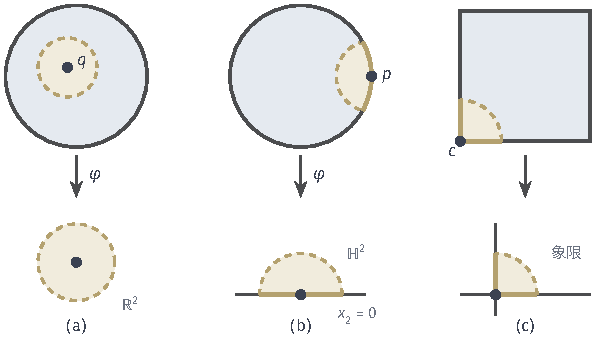
\includegraphics[width=100.856mm]{figures/04-spaces-measures-and-geometry/04-manifolds/tikz/mfd-boundary-models/figure.pdf}
  \caption{三种局部模型。上排是闭圆盘或闭正方形中的一个小邻域（黄），下排是它在坐标图中的像。(a)内点$q$的邻域对应$\mathbb R^2$的开圆盘，虚线表示边不含在内。(b)边界点$p$的邻域对应$\mathbb H^2$的半圆盘，粗黄线是位于边界上的部分，含在邻域内。(c)角点$c$的邻域在平面坐标中是象限，不是半圆盘。}
  \label{fig:mfd-boundary-models}
\end{BookInlineFigure}

\begin{definition}[带边界的拓扑流形]
\label{def:mfd-manifold-with-boundary}
Hausdorff且第二可数的拓扑空间$M$称为$n$维\term{带边界流形}（manifold with boundary），若每个$p\in M$都有开邻域$U$和从$U$到$\mathbb H^n$的某个开子集的同胚$\varphi$。若某张这样的图把$p$送到$\partial\mathbb H^n$中，称$p$为\term{边界点}（boundary point）；若某张图把$p$送到$\{x_n>0\}$中，称$p$为内点。全部边界点组成的集合记为$\partial M$。
\end{definition}

$\{x_n>0\}$本身是$\mathbb R^n$的开集，所以内点附近的局部模型与无边界情形相同。没有边界点的带边界流形就是前面的流形，为了区分，后者也称无边界流形。

\paragraph{半空间上的光滑性}
要定义带边界流形的光滑结构，先得说清半空间开子集上的映射何时光滑。边界点处只有一侧的值，双侧差商算不了偏导数。约定的做法是借助延拓：若映射在边界点附近能光滑地延拓到一个完整的欧氏开邻域，就称它在那里光滑。

\begin{definition}[半空间开子集上的光滑映射]
\label{def:mfd-smooth-halfspace}
设$A\subseteq\mathbb H^n$是开子集，$F:A\to\mathbb R^k$。若对每个$\bm a\in A$，都有$\mathbb R^n$中的开邻域$W\ni\bm a$与光滑映射$\widetilde F:W\to\mathbb R^k$，使$\widetilde F=F$在$W\cap A$上成立，则称$F$光滑。
\end{definition}

延拓不唯一，但边界点处各阶导数与延拓的选择无关。原因在于内点可以逼近边界点：任意边界点$\bm a$都是内点$\bm a+t\bm e_n$（$t\to0^+$）的极限，延拓在这些内点处的导数就是$F$本身的导数，而$\widetilde F$的各阶导数连续，所以在$\bm a$处的值等于内侧导数的极限，由$F$决定。

有了这一定义，带边界流形的光滑相容性、光滑图册和光滑结构可以逐字照搬定义~\ref{def:mfd-smooth-structure}，只是把坐标变换理解为$\mathbb H^n$开子集之间的映射。

\paragraph{内点与边界点不会混淆}
定义~\ref{def:mfd-manifold-with-boundary}说的是“某张图”把点送到边界，于是要问：会不会有一点在一张图中是边界点，在另一张中是内点？直观上，内点四周都有路可走，边界点只有一侧。下面用Jacobian矩阵把这个直观变成证明。

\begin{theorem}[边界点的坐标无关性]
\label{thm:mfd-boundary-invariance}
设$M$是光滑带边界流形，$p\in M$。若某张光滑坐标图把$p$送到$\partial\mathbb H^n$中，则每张包含$p$的光滑坐标图都把$p$送到$\partial\mathbb H^n$中。
\end{theorem}

\begin{proof}
用反证法。设图$(V,\psi)$把$p$送到边界，图$(U,\varphi)$把$p$送到$\{x_n>0\}$。取$\varphi(p)$在$\mathbb R^n$中的开球$W$，使$W\subseteq\varphi(U\cap V)$，这一步用到$\varphi(p)$是内点。记$\tau=\psi\circ\varphi^{-1}$，它在$W$上光滑。

它的逆$\varphi\circ\psi^{-1}$在$\psi(p)$附近光滑，即在$\psi(p)$的欧氏邻域上有光滑延拓$\widetilde\tau$。在$\varphi(p)$附近，$\widetilde\tau\circ\tau=\mathrm{id}$，对它求导得到
\[
\bm J_{\widetilde\tau}(\psi(p))\,\bm J_\tau(\varphi(p))=\bm I_n .
\]
于是$\bm J_\tau(\varphi(p))$可逆。

由局部反函数定理，$\tau$把$\varphi(p)$的某个开邻域映成$\psi(p)$在$\mathbb R^n$中的一个开邻域，该定理可参考\BookChapterRef{chap:implicit-inverse-functions}{卷二第19章“隐函数与反函数”}。可是$\tau$的值都在$\mathbb H^n$中，而$\psi(p)$的最后一个坐标为零，它的任何欧氏开邻域都含有$x_n<0$的点。这一矛盾说明假设不成立。
\end{proof}

对拓扑带边界流形，同样的结论也成立，但证明需要同调等工具，读者可查阅代数拓扑的教材。今后谈论$\partial M$时，总是在光滑情形下进行。

\paragraph{边界本身的结构}
边界点处的坐标图限制到边界上，给出边界的局部坐标。设$(U,\varphi)$是包含边界点的图，由定理~\ref{thm:mfd-boundary-invariance}，
\[
\varphi(U\cap\partial M)=\varphi(U)\cap\partial\mathbb H^n .
\]
把$\partial\mathbb H^n$等同于$\mathbb R^{n-1}$，限制映射$\varphi|_{U\cap\partial M}$就是$\partial M$的一张$n-1$维坐标图。两张这样的图之间的坐标变换是原坐标变换在边界上的限制，仍然光滑。所以$\partial M$是$n-1$维无边界光滑流形。

用闭圆盘检验这些定义。内部的点用平面坐标的限制作图。边界点用极坐标$(\theta,s)$作图，其中$s=1-r\geq0$，例如在$(1,0)$附近取
\[
\theta\in(-\tfrac{\pi}{2},\tfrac{\pi}{2}),\qquad s\in[0,\tfrac12).
\]
在这张图中，圆周恰好对应$s=0$，所以$\partial\overline B{}^2=S^1$，它是一维无边界流形。区间$[0,1]$是一维带边界流形，边界由两个端点组成，是零维流形。

\paragraph{角点不是同一种光滑边界}
闭正方形$[0,1]^2$同胚于闭圆盘，所以是拓扑带边界流形。但在角点处，平面坐标给出的局部模型是象限$\{x_1\geq0,x_2\geq0\}$，而不是半平面。

能否换一张图把象限摊平？把平面看作复平面，$z\mapsto z^2$确实把象限映成上半平面。可它的逆$z\mapsto\sqrt z$在原点不可微，所以这样得到的坐标与平面原有坐标不光滑相容。这说明如果沿用平面坐标所定义的光滑性，角点不能纳入光滑带边界流形的框架。这类对象需要另行建立带角流形的理论，本书不作讨论。

\section{流形的拓扑性质}
\label{sec:mfd-topology}

流形首先是拓扑空间，第~\ref{chap:topological-spaces}章关于连通性与紧性的一般结论都适用。这里只问一个问题：每点附近像欧氏空间这一局部条件，会给整体性质带来什么新结论？下面看两处：连通与路径连通在流形上不再需要区分，紧流形可以用有限张坐标图覆盖。这些结论对带边界流形同样成立，因为半空间中的半球也像欧氏球那样可以用线段连接。

\subsection{连通与路径连通}
\label{sec:mfd-connectedness}

回忆两种概念的区别：连通指空间不能分成两个不相交的非空开集，路径连通指任意两点都能用连续路径连接。路径连通总蕴含连通，反过来一般不成立。

典型反例是拓扑学家的正弦曲线，即曲线$\{(y_1,\sin(1/y_1)):0<y_1\leq1\}$与竖直线段$\{0\}\times[-1,1]$的并，如图~\ref{fig:mfd-connected-sine}(b)所示。曲线越靠近竖直线段振荡越快，竖线上每一点都是曲线上点的极限，所以两部分不能被开集分开，集合连通。但从竖直线段上的点出发，没有连续路径能走到曲线部分。

\begin{BookInlineFigure}
  \centering
  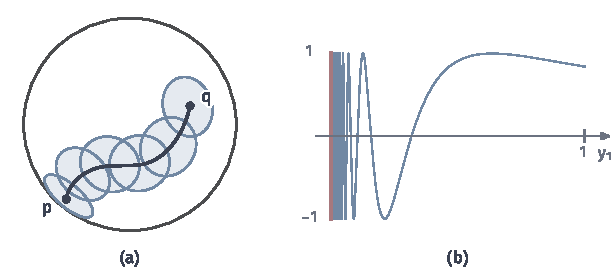
\includegraphics[width=104mm]{figures/04-spaces-measures-and-geometry/04-manifolds/matplotlib/mfd-connected-sine/figure.pdf}
  \caption{局部的线段连接与它失效的情形。(a)球面上连接$p,q$的路径（黑线）由一串相互重叠的坐标球（蓝）接力完成，每个坐标球内部都能用线段走通。(b)拓扑学家的正弦曲线$y_2=\sin(1/y_1)$（蓝）与竖直线段（红）的并。竖线上任意一点的小邻域都含有无穷多段互不相连的弧，所以这里没有路径连通的邻域。}
  \label{fig:mfd-connected-sine}
\end{BookInlineFigure}

\paragraph{局部路径连通}
流形上情况要好得多，因为每点附近都是欧氏的。取包含$p$的坐标图$(U,\varphi)$，在$\varphi(U)$中取以$\varphi(p)$为中心的开球$B$，称$\varphi^{-1}(B)$为\term{坐标球}（coordinate ball）。

球中任意两点$\bm a,\bm b$用线段$t\mapsto(1-t)\bm a+t\bm b$连接，线段留在球内，再用$\varphi^{-1}$送回流形，就得到坐标球内连接两点的连续路径。带边界的情形用半球代替球，半球同样是凸集，线段仍留在其中。于是每点都有任意小的路径连通邻域，这一性质称为\term{局部路径连通}（locally path-connected）。

\begin{theorem}[流形上连通与路径连通等价]
\label{thm:mfd-connected-path-connected}
设$M$是拓扑流形或带边界拓扑流形。则$M$连通当且仅当$M$路径连通。更一般地，$M$的每个路径分支都是既开又闭的集合，并且路径分支与连通分支一致。
\end{theorem}

证明的想法如图~\ref{fig:mfd-connected-sine}(a)：从一点出发能走到的地方，每个点周围都还有一个坐标球能走，所以这个范围不会有“边缘”。

\begin{proof}
设$C$是一个路径分支，即与某点有路径相连的全部点组成的集合。对$q\in C$，取$q$的坐标球$B_q$。$B_q$中每一点都能先连到$q$，再从$q$连到$C$的起点，所以$B_q\subseteq C$，$C$是开集。

不同路径分支互不相交，$C$的补集是其余路径分支的并，也是开集，所以$C$又是闭集。若$M$连通，它唯一的非空既开又闭子集是自身，于是$C=M$，$M$路径连通。反方向是一般拓扑空间中已有的结论。

最后比较两种分支。路径分支$C$路径连通，因而连通，含于某个连通分支$D$。$C$在$D$中既开又闭且非空，$D$连通，所以$C=D$。
\end{proof}

证明只用到“每点有路径连通的邻域”。正弦曲线在竖直线段上的点处缺少这样的邻域，这也说明它不是流形，不能拿来否定定理~\ref{thm:mfd-connected-path-connected}。

\paragraph{连通分支的个数}
每个连通分支是开集，因而本身也是同维流形。第二可数性还限制了分支的个数：每个分支都含有可数基中的某个非空基元素，不同分支所含的基元素不同，所以分支至多可数。

例如双曲线$\{\bm y\in\mathbb R^2:y_2^2-y_1^2=1\}$有上下两个连通分支，每个分支同胚于$\mathbb R$。连通分支数这一整体信息后来由零维同调记录，见第~\ref{chap:homology}章。

\subsection{紧性}
\label{sec:mfd-compactness}

紧空间的任意开覆盖都有有限子覆盖，紧空间上的连续实值函数取得最大值和最小值。这两条在流形上有直接用途。前者让我们只用有限张坐标图处理整个紧流形；后者保证球面上的高度函数$\bm y\mapsto y_3$在某些点达到最高和最低，第~\ref{sec:mfd-smooth-functions}小节将用坐标验证这些点处微分为零。

\paragraph{有限个坐标图}
所有坐标图的定义域组成$M$的一个开覆盖。若$M$紧，就能从中选出有限张图覆盖$M$。圆周用两张图，球面用两张球极投影图，环面用四张乘积图。很多构造先在每张图上局部完成，再把结果拼起来；图的张数有限时，拼接中的求和、取最大值等操作都只涉及有限项。

\paragraph{有限张图不等于一张图}
紧性只给出有限张图，不能推出一张图就够。实际上，正维数的非空紧无边界流形一定不能由单张坐标图覆盖。

证明很短。假设$\varphi:M\to\widehat U$是覆盖整个$M$的坐标图。$\widehat U=\varphi(M)$是紧集的连续像，因而是$\mathbb R^n$中的有界闭集。它又是非空开集，于是是$\mathbb R^n$中非空的既开又闭子集。$\mathbb R^n$连通，所以$\widehat U=\mathbb R^n$，这与有界矛盾。

因此圆周、球面和环面都至少需要两张图。本章开头经纬度在两极失效，问题不在经纬度选得不好，而在于球面的紧性使任何单张坐标图都不可能覆盖全部。

反过来，非紧流形有时一张图就够，例如$\mathbb R^n$。双曲线虽有两个分支，也能用一张图覆盖：在上支令$\varphi(\bm y)=\arctan y_1$，在下支令$\varphi(\bm y)=\arctan y_1+4$，两支分别被送到不相交的开区间$(-\pi/2,\pi/2)$与$(4-\pi/2,4+\pi/2)$。欧氏开集本来就不必连通。单张图能否覆盖整个流形，等于问整个流形能否同胚于一个欧氏开集，紧性只是排除这种可能的一个充分原因。

\section{点与曲线}
\label{sec:mfd-points-curves}

流形是一个整体空间，它的元素是点。在欧氏空间中，点与它的坐标几乎不加区分；在流形上，坐标只是某张局部地图对点的记录，换一张图记录就变。先弄清哪些运算属于点、哪些只属于坐标，再用参数曲线描述点随参数的连续变化。

\subsection{点的坐标表示}
\label{sec:mfd-point-coordinates}

取球面上的点$p=(0,\tfrac35,\tfrac45)$，它就是图~\ref{fig:mfd-stereographic}(b)中的那一点。按式~\eqref{eq:mfd-stereographic-north}，分母是$1-\tfrac45=\tfrac15$，所以北极图坐标是
\[
\sigma_N(p)=\frac{(0,\tfrac35)}{1/5}=(0,3).
\]
按式~\eqref{eq:mfd-stereographic-south}，分母是$1+\tfrac45=\tfrac95$，所以南极图坐标是
\[
\sigma_S(p)=\frac{(0,\tfrac35)}{9/5}=(0,\tfrac13).
\]
两组数不同，记录的是同一个点。代入转移映射\eqref{eq:mfd-stereographic-transition}核对：$\tau(0,3)=(0,3)/9=(0,\tfrac13)$，正好对上。

\paragraph{坐标运算不定义点的运算}
坐标是$\mathbb R^2$中的向量，可以相加。但“两个点的坐标之和”在不同图中对应不同的点。再取$q=(0,-\tfrac35,\tfrac45)$，它在两张图中的坐标分别是$(0,-3)$与$(0,-\tfrac13)$。

两点的坐标相加，在北极图和南极图里都得到$(0,0)$。但$(0,0)$在两张图中代表不同的点：
\[
\sigma_N^{-1}(0,0)=(0,0,-1)=S,\qquad
\sigma_S^{-1}(0,0)=(0,0,1)=N .
\]
同样的两点，用北极图相加得到南极，用南极图相加得到北极。

所以坐标的加法依赖所用的图，不是流形上点的运算。球面上本来也没有自然的加法：$p,q$作为$\mathbb R^3$中向量的和是$(0,0,\tfrac85)$，它根本不在球面上。今后凡是在坐标中做线性运算，都要说明它在哪张图中进行，所得结论是否与图的选择无关。

\paragraph{邻域与点列收敛}
点的接近关系由流形的拓扑决定，坐标图把它如实翻译成欧氏空间中的接近。设$(U,\varphi)$是包含$p$的坐标图。$U$是$p$的开邻域，$\varphi$是同胚，所以$p$在$U$中的邻域与$\varphi(p)$在$\varphi(U)$中的邻域一一对应。点列收敛因此可以逐点翻译成坐标收敛。

\begin{lemma}[点列收敛的坐标判别]
\label{lem:mfd-sequence-convergence}
设$(U,\varphi)$是包含$p$的坐标图，$(p_k)$是$M$中的点列。则$p_k\to p$当且仅当存在$K$，使$k\geq K$时$p_k\in U$，并且$\varphi(p_k)\to\varphi(p)$。
\end{lemma}

\begin{proof}
若$p_k\to p$，因$U$是$p$的开邻域，从某项起$p_k\in U$；$\varphi$连续，所以$\varphi(p_k)\to\varphi(p)$。反过来，若从某项起$p_k\in U$且坐标收敛，因$\varphi^{-1}$连续，$p_k=\varphi^{-1}(\varphi(p_k))\to p$。
\end{proof}

这个判别不依赖图的选择。若$(V,\psi)$是另一张包含$p$的图，从某项起$p_k\in U\cap V$，坐标变换$\psi\circ\varphi^{-1}$连续，所以一张图中的坐标收敛推出另一张图中的坐标收敛。光滑相容比连续更强，它还保证坐标的变化速度在两张图中能够换算，这一点在曲线速度中用到。

引理要求$p_k$最终落入$U$，这一条不能省。圆周上取$p=(1,0)$，令
\[
p_k=\bigl(\cos\tfrac{(-1)^k}{k},\ \sin\tfrac{(-1)^k}{k}\bigr).
\]
用$\theta_1$看，坐标$(-1)^k/k\to0$，所以$p_k\to p$。换用$\theta_2$，偶数项的坐标是$1/k$，奇数项的坐标是$2\pi-1/k$，在区间两端来回跳动。这是因为$p$不在$\theta_2$的定义域内，不说明点列不收敛。

\subsection{光滑曲线}
\label{sec:mfd-smooth-curves}

一个质点在圆周上匀速转动，时刻$t$的位置是$\gamma(t)=(\cos t,\sin t)$。这里的对象是映射$t\mapsto\gamma(t)$，而不只是它经过的点集：同样转过整个圆，转得快慢不同、方向不同，都是不同的运动。

\paragraph{曲线及其光滑性}
曲线是从参数区间到流形的映射。判断它是否光滑，仍然借助坐标：在每一时刻附近，用一张包含当前位置的图记录位置，得到一条普通的欧氏坐标曲线。

\begin{definition}[光滑曲线]
\label{def:mfd-smooth-curve}
设$I\subseteq\mathbb R$是区间，$\gamma:I\to M$连续。若对每个$t_0\in I$和每张包含$\gamma(t_0)$的坐标图$(U,\varphi)$，坐标曲线$\varphi\circ\gamma$在$t_0$附近光滑，则称$\gamma$为\term{光滑曲线}（smooth curve）。$I$含端点时，端点处按单侧导数理解。
\end{definition}

$\gamma$连续，所以$\gamma^{-1}(U)$是包含$t_0$的开集，坐标曲线在$t_0$附近确有定义。定义要求对每张图都成立，但只需检查一张。若$(V,\psi)$是另一张包含$\gamma(t_0)$的图，则在$t_0$附近
\[
\psi\circ\gamma=(\psi\circ\varphi^{-1})\circ(\varphi\circ\gamma).
\]
转移映射光滑，光滑映射的复合仍光滑，所以$\varphi\circ\gamma$光滑推出$\psi\circ\gamma$光滑。对上式用链式法则，就得到两张图中坐标速度的关系：
\begin{equation}
(\psi\circ\gamma)'(t_0)=\bm J\,(\varphi\circ\gamma)'(t_0),\quad
\bm J=\bm J_{\psi\circ\varphi^{-1}}\bigl(\varphi(\gamma(t_0))\bigr).
\label{eq:mfd-curve-velocity-change}
\end{equation}
两张图记录的速度分量不同，但由转移映射的Jacobian矩阵确定地换算。下一节把这种“由一族记录和一条换算规则共同确定的对象”定义为切向量。

\paragraph{圆周上的例子}
在角度图$\theta_1$中，$\gamma(t)=(\cos t,\sin t)$对$t\in(-\pi,\pi)$的坐标曲线是$\theta_1(\gamma(t))=t$；在$\theta_2$中，对$t\in(0,2\pi)$是$\theta_2(\gamma(t))=t$，其余时刻差$2\pi$的整数倍。各段都是一次函数，所以$\gamma$在整条实轴上光滑，两张图记录的速度都是$1$。这与式~\eqref{eq:mfd-curve-velocity-change}一致，因为转移映射是平移，Jacobian为$1$。

\paragraph{曲线与它的像}
同一个像可以由许多不同的曲线描出。曲线$\gamma_2(t)=(\cos2t,\sin2t)$也绕整个圆走，但在角度图中速度为$2$。$\gamma_3(t)=(\cos t^3,\sin t^3)$也绕圆运动，坐标曲线$t^3$光滑，可在$t=0$处速度为零，质点在那一刻停了一下。图~\ref{fig:mfd-curves-parametrization}(a)比较了这三条坐标曲线。

\begin{BookInlineFigure}
  \centering
  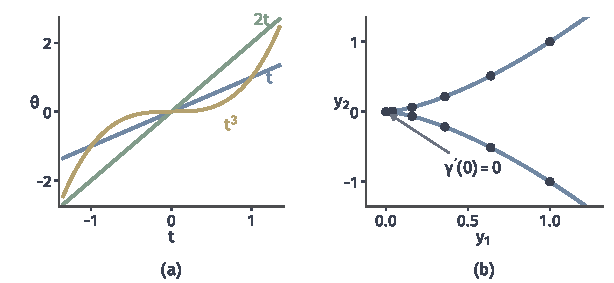
\includegraphics[width=104mm]{figures/04-spaces-measures-and-geometry/04-manifolds/matplotlib/mfd-curves-parametrization/figure.pdf}
  \caption{曲线是映射，不是点集。(a)圆周上三条曲线在角度图中的坐标曲线$\theta=t,2t,t^3$，三者经过相同的点，速度不同，$t^3$在$t=0$处速度为零。(b)平面曲线$\gamma(t)=(t^2,t^3)$的像，黑点是$t=-1,-0.8,\ldots,1$时的位置。分量都是多项式，映射光滑，像却在原点有尖点，那一刻速度恰好为零，黑点也在此处聚拢。}
  \label{fig:mfd-curves-parametrization}
\end{BookInlineFigure}

反过来，映射光滑，像却可以不光滑。平面曲线$\gamma(t)=(t^2,t^3)$的两个分量都是多项式，所以是光滑曲线。计算它的速度：
\[
\gamma'(t)=(2t,\ 3t^2),\qquad \gamma'(0)=(0,0).
\]
它的像$\{(y_1,y_2):y_1^3=y_2^2\}$在原点有尖点，见图~\ref{fig:mfd-curves-parametrization}(b)。尖点处速度恰好为零，所以光滑映射的像才可能在那里拐出尖角。因此“光滑曲线”说的是映射，不是点集；曲线的像能否成为一个光滑子流形，是第~\ref{chap:manifold-relations}章的问题。

\paragraph{边界点处的曲线}
在带边界流形中，曲线可以停在边界上，也可以从边界出发进入内部。闭圆盘中$\gamma(t)=(1-t,0)$，$t\in[0,1)$，从边界点$(1,0)$出发向内运动，只能取$t\geq0$；若取$t<0$，点会离开圆盘。所以过边界点的光滑曲线一般只能是单侧的。

下一节先在内点处用双侧曲线的速度建立切向量。边界点处只收集单侧曲线的速度，得到的是半个空间，而不是线性空间，那里的切空间要换一种方式定义，见第~\ref{sec:mfd-tangent-space}小节。

\section{切空间与余切空间}
\label{sec:mfd-tangent-cotangent}

球面放在$\mathbb R^3$中时，曲线的速度可以直接在$\mathbb R^3$中求导，得到一个与球面相切的向量。一般流形没有现成的外部空间，速度必须用流形自身的语言描述。上一节已经看到，同一速度在两张图中的分量由坐标变换的Jacobian矩阵换算。本节先在内点处把速度定义为曲线的等价类，组成切空间，再用一族坐标记录处理边界点。随后把对切向量的线性读数组织成余切空间，比较两者在换图时的不同变换规则。

\subsection{切空间}
\label{sec:mfd-tangent-space}

\paragraph{内点处的曲线速度}
设$p$是$M$的内点。经过$p$的光滑曲线$\gamma:(-\varepsilon,\varepsilon)\to M$，$\gamma(0)=p$，在一张包含$p$的图$(U,\varphi)$中有坐标速度$(\varphi\circ\gamma)'(0)\in\mathbb R^n$。两条曲线可能形状完全不同，却在$p$处有相同的坐标速度；就“此刻往哪里、以多快的速度运动”而言，它们没有区别。

\begin{definition}[切向量与切空间]
\label{def:mfd-tangent-space}
设$p$是光滑流形$M$的内点，$(U,\varphi)$是包含$p$的坐标图。对经过$p$的两条光滑曲线$\gamma_1,\gamma_2$，若$(\varphi\circ\gamma_1)'(0)=(\varphi\circ\gamma_2)'(0)$，则称二者在$p$处等价。等价类$[\gamma]$称为$p$处的\term{切向量}（tangent vector），也记作$\gamma'(0)$；全体切向量组成的集合$T_pM$称为$M$在$p$处的\term{切空间}（tangent space）。
\end{definition}

定义中用了一张特定的图，但等价关系与图无关：若在$\varphi$中坐标速度相同，由式\eqref{eq:mfd-curve-velocity-change}，在另一张图$\psi$中二者的坐标速度都等于同一个矩阵乘以同一个向量，仍然相同。

\paragraph{切空间的线性结构}
切向量是等价类，本来没有加法。下面借用坐标记录把$\mathbb R^n$的线性结构搬过来，并说明搬来的结构与所用的图无关。

\begin{theorem}[切空间是$n$维线性空间]
\label{thm:mfd-tangent-linear}
设$p$是$n$维光滑流形$M$的内点，$(U,\varphi)$是包含$p$的坐标图。映射
\[
\Theta_\varphi:T_pM\to\mathbb R^n,\qquad [\gamma]\mapsto(\varphi\circ\gamma)'(0)
\]
是双射。用它把$\mathbb R^n$的加法与数乘搬到$T_pM$上，所得线性结构与$\varphi$的选择无关，$T_pM$是$n$维实线性空间。
\end{theorem}

\begin{proof}
单射直接来自等价关系的定义。为证满射，任取$\bm v\in\mathbb R^n$。$p$是内点，$\varphi(U)$是包含$\varphi(p)$的欧氏开集，所以$t$足够小时$\varphi(p)+t\bm v\in\varphi(U)$，曲线$\gamma(t)=\varphi^{-1}(\varphi(p)+t\bm v)$有定义且光滑，坐标速度为$\bm v$。

若$(V,\psi)$是另一张包含$p$的图，式\eqref{eq:mfd-curve-velocity-change}说明$\Theta_\psi=\bm J\,\Theta_\varphi$，其中$\bm J=\bm J_{\psi\circ\varphi^{-1}}(\varphi(p))$是可逆矩阵。可逆线性映射保持线性组合，所以按$\Theta_\varphi$规定的$a[\gamma_1]+b[\gamma_2]$，在$\Theta_\psi$下的记录是$a\Theta_\psi[\gamma_1]+b\Theta_\psi[\gamma_2]$，两张图规定的运算相同。
\end{proof}

\paragraph{坐标基与变换规则}
$\mathbb R^n$的标准基$\bm e_1,\ldots,\bm e_n$在$\Theta_\varphi^{-1}$下给出$T_pM$的一组基，记为
\[
\left.\frac{\partial}{\partial x_i}\right|_p=\Theta_\varphi^{-1}(\bm e_i),\qquad i=1,\ldots,n,
\]
称为\term{坐标基}（coordinate basis），简记为$\partial_i|_p$。它就是第$i$条坐标线$t\mapsto\varphi^{-1}(\varphi(p)+t\bm e_i)$的速度。任一切向量写成$\bm v=\sum_i v_i\,\partial_i|_p$，系数$(v_1,\ldots,v_n)=\Theta_\varphi(\bm v)$称为它在这张图中的分量。

换一张图$\psi$，坐标记为$\tilde x_1,\ldots,\tilde x_n$，同一切向量的分量变为
\begin{equation}
\tilde v_k=\sum_{j=1}^n\frac{\partial\tilde x_k}{\partial x_j}(\varphi(p))\,v_j,
\qquad\text{即}\qquad
\left.\frac{\partial}{\partial x_j}\right|_p=\sum_{k=1}^n\frac{\partial\tilde x_k}{\partial x_j}(\varphi(p))\left.\frac{\partial}{\partial\tilde x_k}\right|_p,
\label{eq:mfd-tangent-change}
\end{equation}
其中$\partial\tilde x_k/\partial x_j$是坐标变换$\psi\circ\varphi^{-1}$的Jacobian矩阵的元素。左式说明分量按Jacobian矩阵变换；右式说明旧的第$j$个基向量由Jacobian矩阵第$j$列的元素组合新基向量得到。两种写法表达同一件事：记录变了，向量本身不变。

\paragraph{球面上的核对}
回到$p=(0,\tfrac35,\tfrac45)$，北极图坐标$\bm u=(0,3)$。对坐标变换$\tau(\bm u)=\bm u/\lVert\bm u\rVert_2^2$求导，得
\[
\bm J_\tau(\bm u)=\frac{\lVert\bm u\rVert_2^2\,\bm I-2\bm u\bm u^\top}{\lVert\bm u\rVert_2^4},\qquad
\bm J_\tau(0,3)=\frac{9\bm I-2\operatorname{diag}(0,9)}{81}=\operatorname{diag}\Bigl(\frac19,-\frac19\Bigr).
\]
于是北极图中的坐标基向量$\partial_{u_1}|_p$，在南极图中的分量是$(\tfrac19,0)$。直接验证：北极图中的坐标线$t\mapsto(t,3)$在南极图中是$t\mapsto(t,3)/(t^2+9)$，在$t=0$处的导数为$(\tfrac19,0)$，与矩阵计算一致。

借助嵌入也可以看到这个切向量的模样。对式\eqref{eq:mfd-stereographic-north}中$\sigma_N^{-1}$关于$u_1$在$(0,3)$处求导，得$\mathbb R^3$中的速度$(0.2,0,0)$，它与$p$的内积为零，确实与球面相切。不过这只是嵌入在$\mathbb R^3$中的球面才有的另一种记录；切空间的定义本身没有用到$\mathbb R^3$。嵌入子流形的切空间怎样作为环境切空间的子空间出现，见第~\ref{chap:manifold-relations}章。

\paragraph{边界点处的切空间}
在边界点$p$处，坐标速度只能从单侧曲线得到，定义~\ref{def:mfd-tangent-space}不再适用。注意式\eqref{eq:mfd-tangent-change}只用到坐标变换在$\varphi(p)$处的Jacobian矩阵，而边界点处的Jacobian矩阵由光滑延拓确定，并且与延拓的选择无关。于是可以绕开曲线，直接用坐标记录及其换算规则定义切向量。

\begin{definition}[用坐标记录定义的切空间]
\label{def:mfd-tangent-records}
设$p\in M$，$M$可以带边界。考虑所有二元组$(\varphi,\bm v)$，其中$\varphi$是包含$p$的坐标图，$\bm v\in\mathbb R^n$。规定
\[
(\varphi,\bm v)\sim(\psi,\tilde{\bm v})\quad\Longleftrightarrow\quad
\tilde{\bm v}=\bm J_{\psi\circ\varphi^{-1}}(\varphi(p))\,\bm v,
\]
其中边界点处的Jacobian矩阵取坐标变换任一光滑延拓的Jacobian矩阵。等价类组成的集合仍记为$T_pM$。
\end{definition}

链式法则说明$\sim$是等价关系：自反性来自恒等变换，对称性来自$\bm J_{\varphi\circ\psi^{-1}}=\bm J_{\psi\circ\varphi^{-1}}^{-1}$，传递性来自三张图之间坐标变换的复合。固定一张图，$\bm v\mapsto[(\varphi,\bm v)]$是$\mathbb R^n$到$T_pM$的双射，与定理~\ref{thm:mfd-tangent-linear}同样的论证给出与图无关的线性结构，坐标基与变换规则\eqref{eq:mfd-tangent-change}照旧成立。在内点处，$[\gamma]\mapsto[(\varphi,(\varphi\circ\gamma)'(0))]$把两种定义一一对应起来，并保持线性运算，所以两种定义可以等同。

\paragraph{完整切空间与单侧方向}
在边界点处，$T_pM$仍然是完整的$n$维线性空间，其中既有指向内部的方向，也有指向外部的方向。这种分类与图无关。

\begin{lemma}[内向与外向的坐标无关性]
\label{lem:mfd-inward-outward}
设$p\in\partial M$，$\varphi,\psi$是包含$p$的两张坐标图，$\tilde{\bm v}=\bm J_{\psi\circ\varphi^{-1}}(\varphi(p))\bm v$。则$\tilde v_n$与$v_n$同为正、同为负或同为零。
\end{lemma}

\begin{proof}
记$\tau=\psi\circ\varphi^{-1}$，它的最后一个分量$\tau_n$在$\mathbb H^n$上非负，并由定理~\ref{thm:mfd-boundary-invariance}在$\partial\mathbb H^n$上为零。沿边界方向求导，$j<n$时$\partial\tau_n/\partial x_j=0$；从内侧求$x_n$方向的单侧导数，$\partial\tau_n/\partial x_n\geq0$。于是Jacobian矩阵的最后一行是$(0,\ldots,0,c)$，$c\geq0$。矩阵可逆，所以$c>0$，$\tilde v_n=cv_n$。
\end{proof}

据此，$v_n>0$的切向量称为内向的，$v_n<0$的称为外向的，$v_n=0$的与边界相切。从$p$出发进入$M$的单侧光滑曲线$\gamma:[0,\varepsilon)\to M$，速度满足$v_n\geq0$；反过来，每个$v_n\geq0$的$\bm v$都是曲线$t\mapsto\varphi^{-1}(\varphi(p)+t\bm v)$在$t\geq0$时的速度。所以单侧曲线的速度恰好组成闭半空间$\{v_n\geq0\}$。它对取负不封闭，不是线性空间，这正是边界点的切空间不能只用实际可行的运动来定义的原因。

闭圆盘在边界点$(1,0)$处可以具体看到这些方向。用第~\ref{sec:mfd-boundary}小节的极坐标图$(\theta,s)$，$s=1-r$。向内运动的曲线$(1-t,0)$在图中是$(\theta,s)=(0,t)$，速度$(0,1)$，内向；绕圆周的运动速度是$(1,0)$，与边界相切；向量$(0,-1)$外向，它属于$T_pM$，却不是圆盘内任何曲线在$p$处的速度。

\subsection{余切空间}
\label{sec:mfd-cotangent-space}

知道一个点在球面上以什么速度运动之后，常常只关心速度的某一方面，例如高度变化得多快，或者沿某个方向的分量是多少。这样的读数对速度是线性的：速度加倍，读数加倍；两个速度相加，读数相加。对切向量的线性读数构成另一个线性空间。

\begin{definition}[余切空间]
\label{def:mfd-cotangent-space}
$p\in M$处切空间的对偶空间$T_p^*M=(T_pM)^*$，即$T_pM$上全体线性泛函组成的空间，称为$M$在$p$处的\term{余切空间}（cotangent space），其元素称为\term{余切向量}（cotangent vector）或协向量。
\end{definition}

有限维线性空间的对偶空间与原空间维数相同，所以$T_p^*M$也是$n$维的。对偶空间、对偶基与对偶映射的一般讨论可参考\BookChapterRef{chap:linear-representation}{卷二第2章“线性空间、映射与坐标”}。

\paragraph{对偶基}
坐标基$\partial_1|_p,\ldots,\partial_n|_p$有唯一的对偶基，记为$\mathrm dx_1|_p,\ldots,\mathrm dx_n|_p$，满足
\[
\mathrm dx_i|_p\bigl(\partial_j|_p\bigr)=\delta_{i,j},\qquad\text{从而}\qquad
\mathrm dx_i|_p(\bm v)=v_i .
\]
所以$\mathrm dx_i|_p$的作用就是读出切向量在这张图中的第$i$个分量。任一余切向量写成$\omega=\sum_i a_i\,\mathrm dx_i|_p$，系数$a_i=\omega(\partial_i|_p)$是它对第$i$条坐标线速度的读数，作用在切向量上为$\omega(\bm v)=\sum_ia_iv_i$。记号$\mathrm dx_i$的来历在第~\ref{sec:mfd-smooth-functions}小节说明：它正是坐标函数$x_i$的微分。

\paragraph{变换规则的比较}
设另一张图中$\omega=\sum_k\tilde a_k\,\mathrm d\tilde x_k|_p$。把$\omega$作用在$\partial_j|_p$上，并用式\eqref{eq:mfd-tangent-change}展开$\partial_j|_p$，得到
\[
a_j=\omega(\partial_j|_p)=\sum_k\frac{\partial\tilde x_k}{\partial x_j}\,\tilde a_k .
\]
记$\bm J$为坐标变换的Jacobian矩阵，$\bm a,\tilde{\bm a}$为两组系数构成的列向量，两种对象的分量变换规则并排写出是
\begin{equation}
\tilde{\bm v}=\bm J\bm v,\qquad \tilde{\bm a}=\bm J^{-\top}\bm a .
\label{eq:mfd-covector-change}
\end{equation}
切向量的分量随$\bm J$变换，余切向量的系数随$\bm J$的逆转置变换。二者配对的结果$\tilde{\bm a}^\top\tilde{\bm v}=\bm a^\top\bm J^{-1}\bm J\bm v=\bm a^\top\bm v$不变，这正是“余切向量是对切向量的读数”应有的性质。

\paragraph{不能未选度量就把二者等同}
在一张图中，切向量$\bm v$与系数相同的余切向量$\bm v^\top$看上去一一对应，很容易把二者当成同一个东西。但这种对应依赖图。仍取$p=(0,\tfrac35,\tfrac45)$，$\bm J=\operatorname{diag}(\tfrac19,-\tfrac19)$。北极图中的切向量$\partial_{u_1}|_p$分量为$(1,0)$，按系数相同对应到余切向量$\mathrm du_1|_p$。

现在把两者都换到南极图。由式\eqref{eq:mfd-covector-change}，切向量的分量变为$(\tfrac19,0)$，余切向量$\mathrm du_1|_p$的系数变为$\bm J^{-\top}(1,0)^\top=(9,0)$。若在南极图中重新按系数相同来对应，切向量$(\tfrac19,0)$对应的余切向量系数是$(\tfrac19,0)$，而不是$(9,0)$。两张图给出的对应不同，所以“系数相同”不是切空间与余切空间之间与图无关的对应。

要在二者之间建立与图无关的对应，需要在每个切空间上额外选定一个内积，把切向量$\bm v$对应到读数$\bm w\mapsto\langle\bm v,\bm w\rangle$。这正是黎曼度量的作用，留到第~\ref{chap:riemannian-geometry}章。本章始终把切向量与余切向量看作两种不同的对象。

\section{流形上的函数与场}
\label{sec:mfd-functions-fields}

切空间和余切空间都是逐点的对象。实际问题中更常见的是随点变化的量：球面上每一点的温度是一个实数，每一点的风速是一个切向量。前者是函数，后者是向量场，把每点的余切向量排在一起又得到协向量场。一条贯穿的界线是：同一点处的值可以相加，不同点处的场值属于不同的线性空间，不能直接比较。

\subsection{光滑函数}
\label{sec:mfd-smooth-functions}

球面上的高度函数$h(\bm y)=y_3$给每一点赋一个实数。要问它是否光滑，仍然把它写进坐标。由式~\eqref{eq:mfd-stereographic-inverse}，高度就是$\sigma_N^{-1}$的第三个分量，于是在北极图中
\begin{equation}
\hat h(\bm u)=h(\sigma_N^{-1}(\bm u))=\frac{\rho-1}{\rho+1},\qquad \rho=\lVert\bm u\rVert_2^2 .
\label{eq:mfd-height-north}
\end{equation}
同样地，记$\tilde\rho=\lVert\bm w\rVert_2^2$，在南极图中
\begin{equation}
\tilde h(\bm w)=\frac{1-\tilde\rho}{1+\tilde\rho}.
\label{eq:mfd-height-south}
\end{equation}
两个表达式都是分母为正的有理函数，所以$h$在每张图中都光滑。

\begin{definition}[流形上的光滑函数]
\label{def:mfd-smooth-function}
设$M$是光滑流形，可以带边界。函数$f:M\to\mathbb R$称为\term{光滑函数}（smooth function），若对每张坐标图$(U,\varphi)$，坐标表示$\hat f=f\circ\varphi^{-1}:\varphi(U)\to\mathbb R$光滑；边界处的光滑性按定义~\ref{def:mfd-smooth-halfspace}理解。全体光滑函数组成的集合记为$C^\infty(M)$。
\end{definition}

与曲线的情形一样，只需在一个图册的每张图中检查：另一张图中的坐标表示等于这里的坐标表示与一个光滑转移映射的复合。光滑函数的和、积、数乘仍光滑，因为坐标表示逐点相加、相乘。

\paragraph{函数的微分}
沿一条曲线观察函数，就得到函数值随时间的变化率。设$p$是内点，$\bm v=[\gamma]\in T_pM$。在图$\varphi$中，$f\circ\gamma=\hat f\circ(\varphi\circ\gamma)$，链式法则给出
\[
(f\circ\gamma)'(0)=\sum_{i=1}^n\frac{\partial\hat f}{\partial x_i}(\varphi(p))\,v_i .
\]
右端只依赖坐标速度$\bm v$，与等价类中代表曲线的选择无关，并且对$\bm v$是线性的。所以它定义了$T_pM$上的一个线性泛函，即一个余切向量。

\begin{definition}[函数的微分]
\label{def:mfd-function-differential}
设$f\in C^\infty(M)$，$p\in M$，$(U,\varphi)$是包含$p$的坐标图。$f$在$p$处的微分是余切向量
\begin{equation}
\mathrm df_p=\sum_{i=1}^n\frac{\partial\hat f}{\partial x_i}(\varphi(p))\,\mathrm dx_i|_p\ \in T_p^*M .
\label{eq:mfd-function-differential}
\end{equation}
对$\bm v\in T_pM$，记$\bm v f=\mathrm df_p(\bm v)$，称为$f$沿$\bm v$的方向导数。
\end{definition}

式~\eqref{eq:mfd-function-differential}用了坐标，需要检查它与图无关。在另一张图中，$\hat f=\tilde f\circ\tau$，其中$\tau$是转移映射。链式法则给出$\nabla\hat f=\bm J^\top\nabla\tilde f$，也就是
\[
\nabla\tilde f=\bm J^{-\top}\nabla\hat f .
\]
这正是余切向量系数的变换规则\eqref{eq:mfd-covector-change}，所以两张图给出同一个$\mathrm df_p$。这一论证不用曲线，因此在边界点处同样适用。

对坐标函数$x_i$本身，坐标表示是$\bm x\mapsto x_i$，偏导数为$\delta_{i,j}$，于是$\mathrm d(x_i)_p=\mathrm dx_i|_p$。这解释了对偶基的记号：$\mathrm dx_i|_p$就是坐标函数$x_i$在$p$处的微分。同样，把坐标基向量作用于函数，得到
\[
\partial_i|_pf=\frac{\partial\hat f}{\partial x_i}(\varphi(p)),
\]
也就是对坐标表示求偏导数。

方向导数满足乘积法则
\[
\bm v(fg)=f(p)\,\bm vg+g(p)\,\bm vf,
\]
因为坐标表示的偏导数满足这一法则。它还只依赖$f$在$p$附近的值：两个函数在$p$的某个邻域上相等，坐标表示在$\varphi(p)$附近相等，偏导数也相等。

\paragraph{球面高度函数的微分}
现在把微分在球面上算一遍，并在两张图中核对。对式~\eqref{eq:mfd-height-north}求偏导，利用$\hat h=1-2/(\rho+1)$，得到
\[
\frac{\partial\hat h}{\partial u_i}=\frac{4u_i}{(\rho+1)^2}.
\]
在$p=(0,\tfrac35,\tfrac45)$处，$\bm u=(0,3)$，$\rho=9$，分母为$100$，于是
\[
\mathrm dh_p=0\cdot\mathrm du_1|_p+\frac{12}{100}\,\mathrm du_2|_p .
\]
读数的含义是：沿$\partial_{u_1}|_p$运动时高度不变，沿$\partial_{u_2}|_p$运动时高度以速率$0.12$变化。前面算过，$\partial_{u_1}|_p$在$\mathbb R^3$中是水平速度$(\tfrac15,0,0)$，它确实不改变高度。

换到南极图。对式~\eqref{eq:mfd-height-south}求偏导，在$\bm w=(0,\tfrac13)$处，$\tilde\rho=\tfrac19$，
\[
\frac{\partial\tilde h}{\partial w_2}=\frac{-4w_2}{(1+\tilde\rho)^2}=-\frac{4}{3}\cdot\frac{81}{100}=-1.08 .
\]
用式~\eqref{eq:mfd-covector-change}从北极图的系数换算，$\bm J^{-\top}=\operatorname{diag}(9,-9)$，得到
\[
\operatorname{diag}(9,-9)\,(0,\ 0.12)^\top=(0,\ -1.08)^\top ,
\]
两种算法一致。图~\ref{fig:mfd-height-rotation}(a)(c)中的蓝圈是高度函数的等高线，标注的数字就是高度值。

\begin{BookInlineFigure}
  \centering
  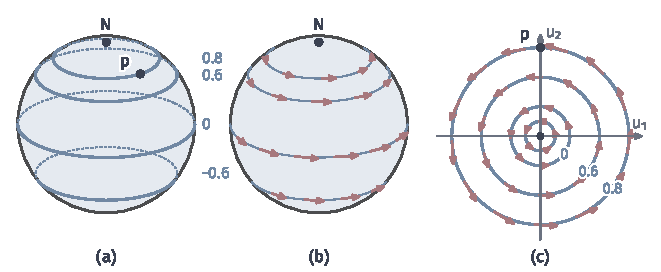
\includegraphics[width=112mm]{figures/04-spaces-measures-and-geometry/04-manifolds/matplotlib/mfd-height-rotation/figure.pdf}
  \caption{球面上的高度函数与旋转场。(a)蓝色纬线是$h=y_3$的等高线，右侧数字是高度，背面用虚线。(b)绕竖直轴的旋转场（红箭头）沿等高线切向，每点的箭头属于该点的切空间。(c)北极图中的同一组对象：半径$r$的圆对应高度$(r^2-1)/(r^2+1)$，半径$\tfrac12,1,2,3$的圆依次对应高度$-0.6,0,0.6,0.8$（最内圈未标数字），红箭头是分量$(-u_2,u_1)$的向量场，长度按比例缩小。}
  \label{fig:mfd-height-rotation}
\end{BookInlineFigure}

在北极，南极图坐标为$\bm w=\bm0$，$\tilde h$的偏导数在$\bm0$处都为零，所以$\mathrm dh_N=0$。这与极值的一般规律相符：若$f$在内点$p$处取局部最大值，则每条经过$p$的曲线$\gamma$使$f\circ\gamma$在$0$处取局部最大值，于是$\bm vf=(f\circ\gamma)'(0)=0$对所有$\bm v$成立，$\mathrm df_p=0$。球面紧，$h$的最大值一定取得，取在北极，微分在那里为零。

注意$\mathrm dh_p$是余切向量，不是一个“梯度方向”。要把它变成指向高度增加最快方向的切向量，需要在切空间上有内积，这一构造在第~\ref{chap:manifold-calculus}章完成。

\subsection{向量场与协向量场}
\label{sec:mfd-vector-covector-fields}

\paragraph{向量场}
设想球面绕竖直轴匀速旋转，每一点都有一个速度，它属于该点的切空间。把这些速度放在一起，就得到一个随点变化、每点取值在不同切空间中的对象，图~\ref{fig:mfd-height-rotation}(b)画的就是它。

\begin{definition}[光滑向量场]
\label{def:mfd-vector-field}
$M$上的\term{向量场}（vector field）$X$给每个$p\in M$指定一个切向量$X_p\in T_pM$。在坐标图$(U,\varphi)$中写成
\begin{equation}
X_p=\sum_{i=1}^nX_i(p)\,\partial_i|_p,\qquad p\in U,
\label{eq:mfd-vector-field-components}
\end{equation}
函数$X_i:U\to\mathbb R$称为$X$的分量。若在每张坐标图中分量都光滑，则称$X$为光滑向量场。$M$上全体光滑向量场的集合记为$\mathfrak X(M)$。
\end{definition}

两张图重叠处，分量按式~\eqref{eq:mfd-tangent-change}逐点变换：
\begin{equation}
\tilde X_k=\sum_{j=1}^n\frac{\partial\tilde x_k}{\partial x_j}\,X_j .
\label{eq:mfd-vector-field-change}
\end{equation}
转移映射的偏导数是光滑函数，所以一张图中分量光滑，另一张图中分量也光滑，只需在一个图册中检查。反过来，若在一个图册的每张图中给定一组光滑函数，并在每个重叠处满足式~\eqref{eq:mfd-vector-field-change}，它们就拼成一个光滑向量场。

\paragraph{协向量场}
同样地，给每点指定一个余切向量，就得到\term{协向量场}（covector field）$\omega$。在图中写成$\omega_p=\sum_ia_i(p)\,\mathrm dx_i|_p$，分量光滑时称为光滑协向量场，重叠处的系数按式~\eqref{eq:mfd-covector-change}变换。最重要的例子是光滑函数的微分：$\mathrm df$在图中的分量是$\partial\hat f/\partial x_i$，光滑，所以$\mathrm df$是光滑协向量场。

\paragraph{例子：球面的旋转场}
绕竖直轴转角$t$的旋转把$\bm y$送到
\[
(y_1\cos t-y_2\sin t,\ y_1\sin t+y_2\cos t,\ y_3),
\]
它不改变$y_3$。由式~\eqref{eq:mfd-stereographic-north}，北极图坐标$\bm u=(y_1,y_2)/(1-y_3)$随之做同一个平面旋转。对$t$在$0$处求导，旋转场在北极图中的分量为
\begin{equation}
(X_1,X_2)=(-u_2,\ u_1).
\label{eq:mfd-rotation-north}
\end{equation}
同理，在南极图中分量为$(-w_2,w_1)$，北极$\bm w=\bm0$处场值为零，这是绕轴旋转时轴上的点不动。

用式~\eqref{eq:mfd-vector-field-change}核对两组分量相容。由式~\eqref{eq:mfd-inversion-jacobian}，先注意$\bm u^\top(-u_2,u_1)^\top=0$，于是
\[
\bm J_\tau(\bm u)\begin{bmatrix}-u_2\\u_1\end{bmatrix}
=\frac{1}{\rho}\begin{bmatrix}-u_2\\u_1\end{bmatrix}.
\]
而$\bm w=\bm u/\rho$，右端恰是$(-w_2,w_1)$。两组分量拼成整个球面上的光滑向量场。

\paragraph{向量场作用于函数}
向量场与函数配合，逐点取方向导数，得到一个新函数：
\begin{equation}
(Xf)(p)=X_pf=\mathrm df_p(X_p).
\label{eq:mfd-field-on-function}
\end{equation}
在坐标图中，$Xf=\sum_iX_i\,\partial\hat f/\partial x_i$。$X$与$f$都光滑时，$Xf$光滑。映射$f\mapsto Xf$是线性的，并满足$X(fg)=f\,Xg+g\,Xf$。

例如旋转场作用于高度函数。由上一小节的偏导数，
\[
Xh=-u_2\cdot\frac{4u_1}{(\rho+1)^2}+u_1\cdot\frac{4u_2}{(\rho+1)^2}=0 .
\]
这符合直观：绕竖直轴旋转不改变高度。图~\ref{fig:mfd-height-rotation}(c)中红箭头沿等高线走，说的是同一件事。

\paragraph{场的逐点运算与不同点的比较}
同一点处的场值属于同一个切空间，所以$X+Y$、$gX$（$g$为光滑函数）可以逐点定义，结果仍是光滑向量场。不同点处的场值却属于不同的切空间，差$X_p-X_q$没有意义。用坐标分量相减看似可行，但结果依赖所选的图。

下面用一个具体计算说明这一点。在北极图中取常值分量的场$X=\partial_{u_1}$，定义在$S^2\setminus\{N\}$上。取$p=\sigma_N^{-1}(0,3)$与$q=\sigma_N^{-1}(1,0)=(1,0,0)$，北极图中两点处的分量都是$(1,0)$，相减为零，看起来是“同一个向量”。

换到南极图。由式~\eqref{eq:mfd-inversion-jacobian}，在$q$处$\bm J_\tau(1,0)=\operatorname{diag}(-1,1)$，于是两点处的分量分别是
\[
p:\ \bm J_\tau(0,3)(1,0)^\top=(\tfrac19,\ 0),\qquad
q:\ \bm J_\tau(1,0)(1,0)^\top=(-1,\ 0).
\]
两者之差不为零。可见“两个不同点处的切向量是否相同”没有与图无关的答案。比较不同点的方向需要额外的搬运规则，这是第~\ref{chap:riemannian-geometry}章联络与平行移动的任务。

\subsection{向量场的Lie括号}
\label{sec:mfd-lie-bracket}

向量场可以先后作用于函数。$Y$作用于$f$得到函数$Yf$，$X$再作用得到$X(Yf)$，交换次序得$Y(Xf)$。在欧氏空间中，常系数的偏导数可以交换次序；系数随点变化时，两种次序一般不同。这个差既不依赖度量，也有清楚的运动含义。

\paragraph{交换差仍是向量场}
两个一阶导数的复合本来是二阶算子，先写出来看。在坐标中记$X=\sum_iX_i\partial_i$，$Y=\sum_jY_j\partial_j$，$\hat f$为$f$的坐标表示，由乘积法则，
\[
X(Yf)=\sum_{i,j}X_i\,(\partial_iY_j)\,\partial_j\hat f+\sum_{i,j}X_iY_j\,\partial_i\partial_j\hat f .
\]
$Y(Xf)$的展开相同，只是$X,Y$对调。二阶偏导数可交换，两式中的二阶项相同，相减时抵消，只剩一阶项：
\begin{equation}
X(Yf)-Y(Xf)=\sum_{j=1}^n\Bigl(\sum_{i=1}^n\bigl(X_i\,\partial_iY_j-Y_i\,\partial_iX_j\bigr)\Bigr)\partial_j\hat f .
\label{eq:mfd-lie-bracket-coordinates}
\end{equation}
右端是某个向量场作用于$f$的结果，它的分量是括号中的光滑函数。

\begin{definition}[Lie括号]
\label{def:mfd-lie-bracket}
对$X,Y\in\mathfrak X(M)$，由
\begin{equation}
[X,Y]f=X(Yf)-Y(Xf)
\label{eq:mfd-lie-bracket-def}
\end{equation}
确定的向量场$[X,Y]$称为$X$与$Y$的\term{Lie括号}（Lie bracket）。在坐标图中，它的分量由式~\eqref{eq:mfd-lie-bracket-coordinates}给出。
\end{definition}

还要说明不同图中的分量拼成同一个向量场。在图$\varphi$中把式~\eqref{eq:mfd-lie-bracket-coordinates}定义的场记为$Z$，在图$\psi$中记为$\tilde Z$。二者在重叠处作用于任意光滑函数，都等于与图无关的$X(Yf)-Y(Xf)$。

把$f$取为第二张图的坐标函数$\tilde x_k$（只在重叠的开集上用，方向导数只依赖函数在点附近的值），得到
\[
\tilde Z_k=Z\tilde x_k=\sum_{j=1}^n Z_j\,\frac{\partial\tilde x_k}{\partial x_j},
\]
这正是变换规则\eqref{eq:mfd-vector-field-change}。

\paragraph{一个计算例子}
在$\mathbb R^2$上取$X=\partial_1$，$Y=x_1\partial_2$。由式~\eqref{eq:mfd-lie-bracket-coordinates}，$[X,Y]$的第二个分量是$X_1\partial_1Y_2=1$，其余为零，所以
\[
[X,Y]=\partial_2 .
\]
对函数直接核对。两种先后次序分别是
\[
X(Yf)=\partial_1(x_1\partial_2f)=\partial_2f+x_1\partial_1\partial_2f,\qquad
Y(Xf)=x_1\partial_2\partial_1f .
\]
相减得$\partial_2f$，与上面一致。

这个结果可以从运动的角度理解。沿$X$走时间$\varepsilon$是向右平移$\varepsilon$；沿$Y$走时间$\varepsilon$是把$(a,b)$变为$(a,b+\varepsilon a)$，向上移动的距离取决于当时的横坐标。从$(a,b)$出发，两种走法的终点分别是
\[
\text{先}X\text{后}Y:\ (a+\varepsilon,\ b+\varepsilon a+\varepsilon^2),\qquad
\text{先}Y\text{后}X:\ (a+\varepsilon,\ b+\varepsilon a).
\]
两条路线的终点相差$(0,\varepsilon^2)$，是二阶小量，方向正是$\partial_2$。Lie括号度量的就是两种运动先后次序不可交换的程度，图~\ref{fig:mfd-lie-bracket}画出了这两条路线。

\begin{BookInlineFigure}
  \centering
  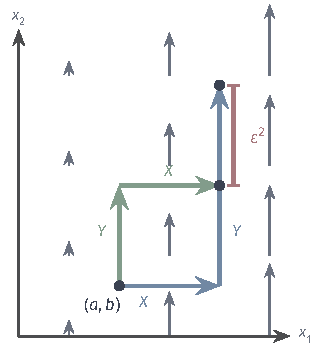
\includegraphics[width=54.906mm]{figures/04-spaces-measures-and-geometry/04-manifolds/tikz/mfd-lie-bracket/figure.pdf}
  \caption{Lie括号是运动次序的差。灰色箭头是场$Y=x_1\partial_2$，越往右越长。从$(a,b)=(1,\tfrac12)$出发，取$\varepsilon=1$：蓝色路线先沿$X=\partial_1$再沿$Y$，绿色路线先沿$Y$再沿$X$，终点相差红色线段$\varepsilon^2=1$，方向是$[X,Y]=\partial_2$。蓝色路线走$Y$时横坐标已经变大，所以走得更高。}
  \label{fig:mfd-lie-bracket}
\end{BookInlineFigure}

\paragraph{基本性质}
由定义直接可得反对称性与线性，对实数$a,b$和光滑函数$g$有
\[
\begin{gathered}
[X,Y]=-[Y,X],\qquad [aX+bY,Z]=a[X,Z]+b[Y,Z],\\
[X,gY]=g[X,Y]+(Xg)Y .
\end{gathered}
\]
此外还有Jacobi恒等式
\[
[X,[Y,Z]]+[Y,[Z,X]]+[Z,[X,Y]]=0,
\]
把三项都作用于$f$并按定义展开，得到十二个三阶复合项，它们两两抵消。坐标基向量场的Lie括号为零，$[\partial_i,\partial_j]=0$，这正是二阶偏导数可交换。

Lie括号的定义只用到向量场作用于函数，不需要先选度量或联络。第~\ref{chap:riemannian-geometry}章用它表述联络的无挠条件与曲率，第~\ref{chap:lie-groups}章用它刻画连续变换群在单位元附近的结构。

\section{光滑单位分解}
\label{sec:mfd-partition-unity}

很多构造在一张坐标图里很容易完成，例如在坐标中写下一个函数、一个向量场或一个内积。但整个流形通常需要多张图，各图上的构造在重叠处一般不一致，不能直接拼接。办法是给每张图配一个光滑权重，只在该图内部取正值，所有权重之和处处为一；各图上的构造乘以权重后相加，在每点附近只涉及有限项，结果就是整体上光滑的对象。本节构造这样的权重。

\paragraph{支撑受限的光滑函数}
第一步要有在一个区域外恒为零、在区域内为正的光滑函数。多项式做不到这一点：非零多项式不能在一个区间上恒为零。下面的函数在原点处以所有阶导数为零的方式“起飞”：
\begin{equation}
\eta(t)=\begin{cases}e^{-1/t},&t>0,\\0,&t\leq0.\end{cases}
\label{eq:mfd-smooth-step}
\end{equation}
当$t>0$时，$\eta$的$k$阶导数形如$P_k(1/t)e^{-1/t}$，$P_k$是多项式；令$s=1/t\to+\infty$，$P_k(s)e^{-s}\to0$，所以各阶导数从右侧趋于零，与左侧的零函数衔接，$\eta$在$\mathbb R$上光滑。

用$\eta$可以造出欧氏空间中的光滑截断函数。对$0<r<R$，令
\[
\chi(\bm x)=\frac{\eta(R^2-\lVert\bm x\rVert_2^2)}{\eta(R^2-\lVert\bm x\rVert_2^2)+\eta(\lVert\bm x\rVert_2^2-r^2)} .
\]
分母的两项不会同时为零，因为$\lVert\bm x\rVert_2^2<R^2$与$\lVert\bm x\rVert_2^2>r^2$至少有一个成立。于是$\chi$光滑，取值在$[0,1]$中，在半径$r$的闭球上恒为$1$，在半径$R$的球外恒为$0$。这类函数称为\term{截断函数}（cutoff function）。

函数$f$的\term{支撑}（support）是集合$\{p:f(p)\neq0\}$的闭包，记为$\operatorname{supp}f$。取闭包是为了让“$f$在支撑之外恒为零”成为开集上的性质：$\chi$的支撑是半径$R$的闭球。把$\chi$放进一张坐标图，并乘到坐标表示上，就能把局部构造截断成在整个流形上有定义的函数，前提是截断后的支撑落在图的定义域内部。

\paragraph{局部有限的覆盖}
多个权重相加时，若每点附近有无穷多个权重非零，和可能不收敛，也可能不光滑。所以需要覆盖满足局部有限条件。设$\{V_\beta\}$是$M$的一族子集，若每点都有一个邻域只与其中有限个$V_\beta$相交，则称这族子集\term{局部有限}（locally finite）。若一个开覆盖$\{V_\beta\}$的每个成员都含于给定开覆盖$\{U_\alpha\}$的某个成员中，则称前者是后者的一个\term{细化}（refinement）。

\begin{definition}[光滑单位分解]
\label{def:mfd-partition-unity}
设$\{U_\alpha\}_{\alpha\in A}$是$M$的开覆盖。一族光滑函数$\{\psi_\alpha\}_{\alpha\in A}$称为从属于$\{U_\alpha\}$的光滑\term{单位分解}（partition of unity），若：
\begin{enumerate}
\item 对每个$\alpha$，$0\leq\psi_\alpha\leq1$且$\operatorname{supp}\psi_\alpha\subseteq U_\alpha$；
\item 支撑族$\{\operatorname{supp}\psi_\alpha\}$局部有限；
\item 对每个$p\in M$，$\sum_{\alpha}\psi_\alpha(p)=1$。
\end{enumerate}
\end{definition}

由局部有限性，每点附近只有有限个$\psi_\alpha$不为零，所以第三条中的和在每点附近是有限和，自然光滑。

\paragraph{一维的例子}
在$\mathbb R$上取开覆盖$U_1=(-\infty,1)$、$U_2=(-1,\infty)$。令
\[
\psi_1(x)=\frac{\eta(\tfrac12-x)}{\eta(\tfrac12-x)+\eta(x+\tfrac12)},\qquad
\psi_2(x)=\frac{\eta(x+\tfrac12)}{\eta(\tfrac12-x)+\eta(x+\tfrac12)} .
\]
对每个$x$，$x<\tfrac12$与$x>-\tfrac12$至少有一个成立，分母为正。两函数都光滑，取值于$[0,1]$，和为$1$。$\psi_1$的支撑是$(-\infty,\tfrac12]$，含于$U_1$；$\psi_2$的支撑是$[-\tfrac12,\infty)$，含于$U_2$。

这里特意把截断点取在$\pm\tfrac12$而不是$\pm1$。若用$\eta(1-x)$，支撑就是$(-\infty,1]$，不含于开集$U_1$。支撑必须严格落在开集内，乘上权重的局部构造才能在开集的边缘以外光滑地补零。

\paragraph{存在定理}
单位分解的存在要用到流形定义中的全部条件：局部欧氏性提供坐标球上的截断函数，Hausdorff性与第二可数性保证能把覆盖细化为局部有限的。

\begin{theorem}[光滑单位分解的存在]
\label{thm:mfd-partition-unity-existence}
设$M$是光滑流形，可以带边界，$\{U_\alpha\}_{\alpha\in A}$是$M$的任一开覆盖。则存在从属于$\{U_\alpha\}$的光滑单位分解。
\end{theorem}

\begin{proof}
先处理$M$紧的情形，它已包含构造的全部想法。对每个$p\in M$，取包含$p$的坐标图$(V,\varphi)$与某个$U_\alpha\ni p$，在$\varphi(V\cap U_\alpha)$中取以$\varphi(p)$为中心、半径为$R_p$的球，其闭包仍在其中。令$B_p$为半径$R_p/2$的同心球在$\varphi^{-1}$下的原像。边界点处用半球代替球，下同。

$\{B_p\}$覆盖$M$，由紧性可选出有限个$B_{p_1},\ldots,B_{p_m}$覆盖$M$。对每个$k$，取截断函数$\chi_k$，在半径$R_{p_k}/2$的闭球上为$1$，在半径$\tfrac34R_{p_k}$的球外为$0$。令$\lambda_k=\chi_k\circ\varphi_k$在图内，图外为$0$。$\lambda_k$的支撑是半径$\tfrac34R_{p_k}$的闭球的原像，它是紧集，在Hausdorff空间中是闭集，所以图外补零后$\lambda_k$在$M$上光滑。

$\lambda_k\geq0$，并在$B_{p_k}$上等于$1$，所以$\Lambda=\sum_k\lambda_k$处处至少为$1$。令$\tilde\psi_k=\lambda_k/\Lambda$，它们光滑、非负、和为一，且每个$\tilde\psi_k$的支撑含于某个$U_{\alpha(k)}$。最后对每个$\alpha$令$\psi_\alpha=\sum_{k:\alpha(k)=\alpha}\tilde\psi_k$，空和取$0$，就得到以原指标集编号的单位分解。

一般情形只需把“选有限个$B_p$”换成“选局部有限的可数个”。第二可数性与局部欧氏性给出一列紧集$K_1\subseteq K_2\subseteq\cdots$，满足$K_j$含于$K_{j+1}$的内部且$\bigcup_jK_j=M$。对每个$j$，紧集$K_{j+1}\setminus\operatorname{int}K_j$可用有限个如上的坐标球覆盖，并让这些球含于$\operatorname{int}K_{j+2}\setminus K_{j-1}$。每点只与相邻几层的球相交，所以全部球组成局部有限的覆盖，其余步骤与紧情形相同。紧集列的构造这里不展开，它是第二可数局部紧Hausdorff空间的一般性质。
\end{proof}

\paragraph{单位分解的用途}
单位分解的典型用法是“局部构造，加权求和”。设$f_\alpha$是定义在$U_\alpha$上的光滑函数，则$\sum_\alpha\psi_\alpha f_\alpha$在整个$M$上有定义并且光滑，其中每项在$U_\alpha$外按零理解。若所有$f_\alpha$在某点附近都等于同一个值，加权和在那里也等于这个值，因为权重之和为一。

由此可得两个直接结论。第一，任一点$p$的任一邻域中都有光滑函数在$p$附近等于某个给定的局部光滑函数，在邻域外为零；这说明局部定义的坐标函数可以截断成全局光滑函数，切向量完全由它对全局光滑函数的作用确定。第二，在每张图中取欧氏内积，用单位分解加权相加，就在每个切空间上得到一个内积。正定性在加权求和下保持，因为每点处的权重非负、和为一，至少有一项严格为正。这正是第~\ref{chap:riemannian-geometry}章黎曼度量存在的依据。同样的手法也用于把局部坐标中的积分拼成流形上的积分，见第~\ref{chap:manifold-calculus}章。

\section{本章小结}
\label{sec:mfd-summary}

本章开头的问题是：经纬度在两极失效、角度绕圆一周会跳跃，这样的对象应当怎样记录？回答是放弃单张全局坐标，改用一族局部坐标图，并要求重叠处的转移映射光滑可逆。圆周的转移映射是平移，球极投影的转移映射是反演$\bm u/\lVert\bm u\rVert_2^2$，环面的转移映射是圆周转移映射的并排。

流形因此是一个整体空间：Hausdorff且第二可数，每点附近同胚于欧氏开集。光滑结构由光滑相容的坐标图决定，同一拓扑空间上可以有不同的光滑结构，例如$\mathbb R$上$x\mapsto x^3$给出的图与恒等图不相容。允许局部模型为半空间，就得到带边界流形；边界点的身份与图无关，边界本身是低一维的无边界流形，带角点的集合不属于这种光滑边界情形。

局部欧氏结构使流形的整体拓扑比一般拓扑空间规整。坐标球路径连通，所以路径分支都是既开又闭的，连通与路径连通等价；第二可数性又使连通分支至多可数。紧流形可以用有限张图覆盖，但正维数的紧无边界流形不能只用一张图，球面上的经纬度困难正源于此。

本章区分了三个层次的对象，表~\ref{tab:mfd-summary-records}用球面上的点$p=(0,\tfrac35,\tfrac45)$把它们并排列出。点是空间的元素，坐标的加法依赖图，不是点的运算。切向量是曲线速度的等价类，分量按转移映射的Jacobian矩阵变换；边界点处切空间用坐标记录定义，单侧可行的方向只占其中的半空间。余切向量是切向量的线性读数，系数按Jacobian矩阵的逆转置变换，在选定度量之前不能与切向量等同。

\begin{BookInlineTable}
  \centering
  \begin{tabular}{llll}
    \toprule
    对象 & 北极图 & 南极图 & 换算\\
    \midrule
    点$p$ & $(0,3)$ & $(0,\tfrac13)$ & $\tau$\\
    切向量$\partial_{u_1}|_p$ & $(1,0)$ & $(\tfrac19,0)$ & $\bm J$\\
    余切向量$\mathrm dh_p$ & $(0,0.12)$ & $(0,-1.08)$ & $\bm J^{-\top}$\\
    \bottomrule
  \end{tabular}
  \caption{球面上同一组对象在两张图中的记录，其中$\bm J=\operatorname{diag}(\tfrac19,-\tfrac19)$。}
  \label{tab:mfd-summary-records}
\end{BookInlineTable}

随点变化的对象在坐标中由分量记录，分量光滑即对象光滑。光滑函数的微分$\mathrm df_p$是余切向量，内点处的局部极值点微分为零。向量场作用于函数得到方向导数，两个向量场先后作用的交换差是一阶算子，给出Lie括号，它不依赖度量或联络。同一点的场值可以运算，不同点处的场值属于不同的切空间，坐标分量之差依赖图，不能当作它们的比较。光滑单位分解把各图上的构造加权拼成整体，依赖流形定义中的全部条件。

这些都是单个流形内部的结构。点从一个流形映到另一个流形时，切向量与余切向量怎样随之改变，是第~\ref{chap:manifold-maps}章的问题；比较不同点处的方向、度量长度和距离，要在第~\ref{chap:riemannian-geometry}章引入黎曼度量与联络。

